%% !TeX root = ./introduction.tex
%% !TEX TS-program = xelatex
%% !TEX encoding = UTF-8 Unicode

% 系统简介
\chapter{简介}


\large{LMALPHA}\footnote{LMALPHA:Alpha因子设计与执行系统名称。}
\normalsize\phantom{L}
是辅助研究员与开发员设计验证Alpha策略的一套软件系统。\\

系统主要功能特征是简化Alpha因子模型设计与验证流程,主要技术特征是实现高性能执行
因子计算与分析。\\

系统由数据子系统、因子计算函数库、辅助函数库、调用管理程序、分析结果仪表盘
程序等5个子系统组成。\\

系统支持结构化数据与非结构化数据访问、支持常用统计与计算函数、支持后台批处理模式
连续运行。\\

形象来说,将一个策略想法轻松变成可以高性能运行的验证程序,研究员将会获得极大的灵活性和
工作效能。而痛苦的中间过程需要经历分析、设计、编码、调试、部署与运行等诸多环节,其中还
包括掌握计算机体系结构知识、数据库知识、CPP语言知识、程序设计知识、各类周边库知识、
数学工具与模型知识等等。通过LMAlpha,让掌握模型知识的研究员不假程序员之手编写高性能
因子计算程序成为可能。\\

\large{主要功能}\normalsize{}——\\

实现快速验证Alpha因子,给研究员与基金管理人员提供及时可靠的策略执行与策略调整的量化依据。


%设计原理
\chapter{设计原理}

\large{系统设计一般原理}\normalsize{}\\

一切系统设计的出发点,首先就要有正确的目标定位。系统设计的差异性,核心表现在不同系统的主要矛盾
的差异性上--也即是抓系统主要特性。更进一步,在现在以及可预见的未来,量化分析已经且仍会是交易领域
主流共识的这一共性条件下,系统设计应强调那一方面能力,将决定我们在这个领域最终的市场表现--也即
交易领域的技术认识。\\

对于LMAlpha系统,目标定位是满足研究员对因子验证程序的便捷化开发与高性能执行。同时提升开发效率
与执行效率—— 一切系统设计皆须从此出发点开展。\\

而开发效率与执行效率的矛盾恰好是通用程序设计语言的主要矛盾,系统要提升效率,需要在“通用”二字上
做足文章,方法就是引入领域概念与领域模型\footnote{领域概念与领域模型:Domain Specified
Modeling,提供对相关领域概念与对象的抽象与封装,简化设计人员的对领域问题的规划与描述难度。}
,通过牺牲部分通用性而强调和突出特定功能。
变通用为专用——系统主要特性设计从此处展开。\\

在功能设计与约束条件发生冲突时,系统设计做不到开发与执行效率得而兼之,取舍之间的道理不会是一成
不变,不变的原理是设计依据需要符合交易领域的技术发展逻辑。我们对交易领域设计技术与执行
技术的认识和发展展望——规范系统一般性设计依据。\\

考虑到alpha项目开展的风险较大,并且项目需求与系统功能还没有明确一个清晰的完整的定义,因此系
统设计一定要符合当前实际需求,按照需求实际通过迭代式方法设计与实现系统,当需求切实发生变动时实
时修改设计。
KISS原则\footnote{KISS原则: Keep It Simple and Stupid, 不是不要优化系统,而是要避免过度优
化和过早优化。}
加Agile原则\footnote{Aglie原则: 敏捷设计犹如动态规划算法,在设计迭代过程中,每一步选取最优
方案,从而达到全局最优。}
——采用增量化设计技术,同时避免过度的设计。 \\


\large{总结}\normalsize{}
\begin{enumerate}
\item 同时提升开发效率与执行效率----系统设计皆须从此出发点开展。
\item 变通用为专用----系统主要特性设计从此处展开。
\item 符合我们对交易领域设计技术与执行技术的认识和发展展望----规范系统一般性设计依据。
\item KISS原则加Agile原则--采用增量化设计技术,同时避免过度的设计。
\end{enumerate}

——以上。


\section{状态机}

描述系统活动视图,TBD。

\section{框架与库}
描述系统组成与功能视图,TBD。

\chapter{总体设计}

\section{LMAlpha总体设计}

\footnote{立场:通过软件手段与系统技术满足永无止境的因子设计与策略验证需要。}
基本需求来源于永无止境的因子设计与策略验证需要。我们通过引入新的软件手段与系统技术,不断
设计与重构本系统以服务于这个需求。\\

\footnote{观点:系统服务于研究员与交易员的工作需要。}
基本观点是改进目前的因子验证与策略设计方法。Alpha因子设计的主要目的是实现研究思路的快
速验证,提高研究员效率,同时也可以作为交易过程中
策略验证与改进的辅助手段。\\

\footnote{方法:基于C++语言基础环境实现领域化系统设计。}
基本方法是引入其他领域成熟技术结合本领域的需求实际。Alpha策略应用前景非常看好,
进而带动了对因子与策略设计验证的系统需求。基于C++的软件设计开发,由于其
开发效率与执行效率相对均较高,提供复杂系统抽象与封装的设计方法等特性,是目前乃至未来一段时间内
主要的高性能开发通用程序语言。提高因子计算性能既提高Alpha策略的研究能力,能为基于Alpha策略
的交易提高市场机会。在另一方面,通过引入领域概念与领域模型等元语言技术
\footnote{元语言:Meta Language,简单来说就是构建语言的语言},研究员可以使用自己熟悉的
概念与术语直接操作系统,将极大简化软件使用学习与编程难度,从而提高因子研究的效率。
\\

系统总的设计的主要目的是服务于因子设计,主要特性是高效率\footnote{这里效率指的总体效率,
包含因子的开发效率和执行效率}。\\

\section{需求与分析}

第一阶段系统设计依据的用户需求列表,如图\ref{fig:s1-userstories}所示。需求总体可以分为
功能性需求与非功能性需求两大类。其中功能性需求有6个,包含1个规范技术标准和其他5个需
要设计开发的功能。非功能性需求有3个,包含1个项目管理规范和其他2个需要执行项目管理的需求。\\

系统需求勾画了系统的三个基本组成部分与工作模式,如图\ref{fig:s1-system_structure}所示。系统划分为三个子系统,项目管理,配置管理与协同工作。 \\


系统工作模式采用每日Scrum\footnote{Scrum: IEEE Scrum是敏捷开发的一种国际标准。}方式
组织与开展,它连通协同工作与项目管理,而项目管理则同时辅助配置管理。通过协同工作,实现项目状态同步,并将当日发生的问题反馈到开发者,以便于更新设计。\\



\section{功能设计目标}

基于对需求的分析,第一阶段的设计目标是实现一个最小化的验证系统。系统规范技术开发标准
,包括统一使用VS2015
\footnote{VS2015:Visual Studio 2015,微软公司开发工具环境。}集成开发环境,
工程字符串处理采用Unicode编码格式,编译目标架构是x64环境等等。系统因子开发通过VS2015进行,不
再单独设计因子开发程序。剩余功能需求和与之相对应的设计目标如下:



\begin{enumerate}

\item 实现最基本的因子执行功能——设计基于UI
\label{func_ui}
\footnote{UI:User Interface,用户交互界面。}
的因子模型调用模块。

\item 实现最基本的数据计算功能——设计包含线性回归函数与残差计算功能的因子设计辅助模块。
\label{func_lmlib}

\item 实现最基本因子开发功能——设计基于C++11标准高层调用接口API模块。
\label{func_lmapi}

\item 实现最基本因子结果展示功能——设计基于Excel+Python的分析模版,实现因子计算结果数据的
快速查询分析与可视化图表展示。
\label{func_dashboard}
\end{enumerate}

\begin{figure}[ht]
\centering
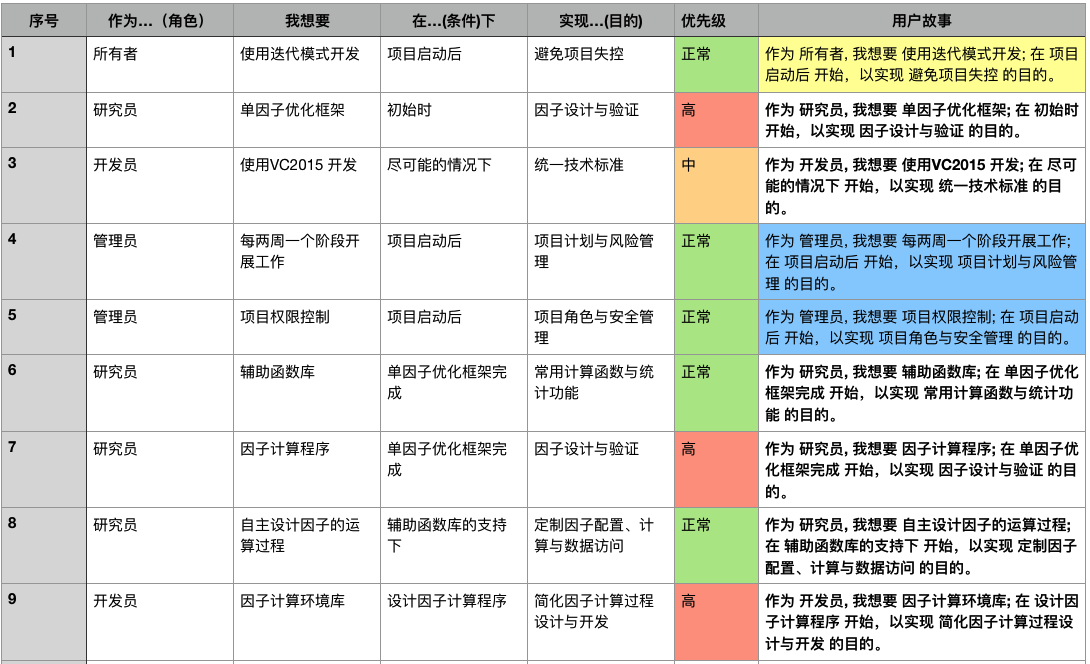
\includegraphics[width=14cm]{sprint1-userstories.png}
\caption{LMAlpha系统sprint1期间用户需求}
\label{fig:s1-userstories}
\end{figure}

\begin{figure}[ht]
    \centering
    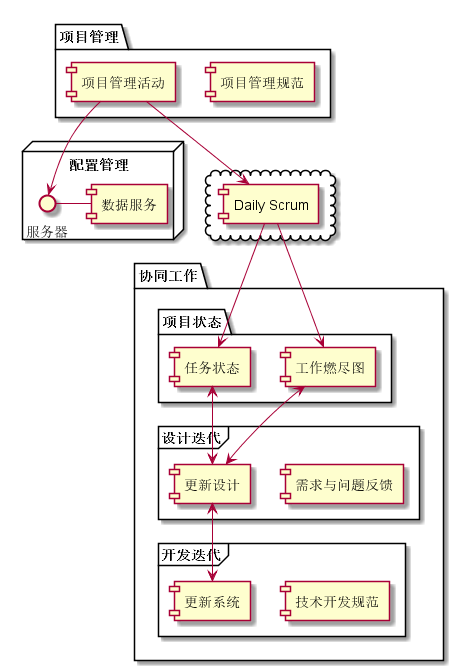
\includegraphics[height=10cm]{system_structure.png}
    \caption{LMAlpha系统组成与工作模式}
    \label{fig:s1-system_structure}
\end{figure}



\section{系统设计的项目约束}

系统功能划分来源于两次面对面沟通,第一阶段预计开发时间为1周,开发团队4人,主要功能实现1人,如图
\ref{fig:s1-teamview}所示。
因此不得不考虑压缩需求和简化设计实现。 \\

\begin{figure}[ht]
\centering
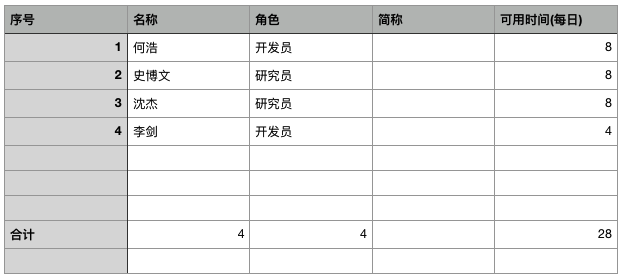
\includegraphics[width=14cm]{sprint1-teamview.png}
\caption{LMAlpha系统sprint1团队一览}
\label{fig:s1-teamview}
\end{figure}

\section{系统功能设计调整}

对于功能需求\ref{func_ui},在设计时不得不舍去GUI\footnote{GUI:Graphics User Interface,图形用户界面。}目标,转而去设计实现更简单的CUI\footnote{CUI:Console User Interface,控制台用户界面。}。\\

对于功能需求\ref{func_lmlib},在设计时考虑放弃对TA-lib的封装,转而对更为广泛使用的GSL库
的封装。\\

对于功能需求\ref{func_lmapi},在设计时并没有更多领域概念与领域模型考虑,仅使用C++语言完成
5类基础功能的API接口封装。\\

对于功能需求\ref{func_dashboard},没有硬性做为本阶段设置目标要求。

\section{项目管理设计}

基于对需求的分析,第一阶段的项目管理目标是摸索一套有效满足项目管理规范,且方便各方理解掌握
与参与的项目管理工具与活动。系统依据的项目管理规范主要考虑风险管理需要与安全管理需要,因此
严格文档及代码的使用和访问范围。项目管理工具的设计,主要基于Excel开发包含三个视图的轻
量化管理模版。
\begin{enumerate}

\item 用户故事——设计规范化的用户需求生成结构。
如\ref{fig:s1-p-userstories}所示。

\item 工作内容——设计对应用户故事的工作任务表,以便于协同工作和状态追踪。
如图\ref{fig:s1-p-backlog}所示。

\item 燃尽图——设计基本统计指标和图表管理项目风险与目标。
如图\ref{fig:s1-p-burndown}所示。

\end{enumerate}

\begin{figure}[htbp]
\centering
\subfigure[用户故事]{
\begin{minipage}[t]{0.32\linewidth}
\centering
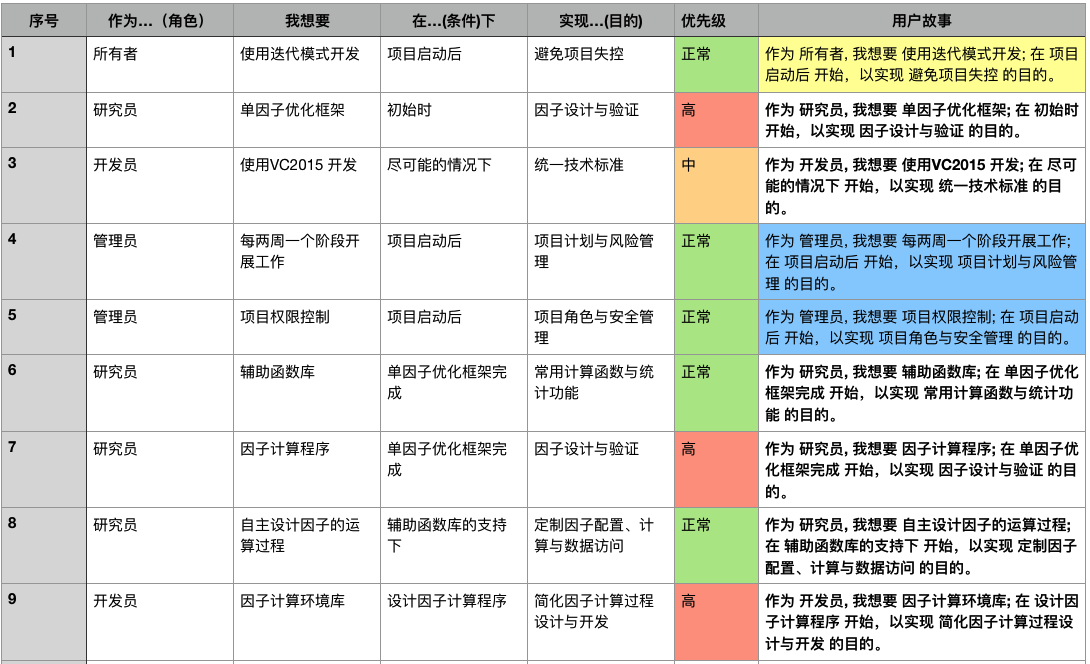
\includegraphics[width=5cm,height=4cm]{sprint1-userstories.png}
\label{fig:s1-p-userstories}
% \caption{LMAlpha系统sprint1工作任务表}
\end{minipage}%
}%
\subfigure[工作任务]{
\begin{minipage}[t]{0.32\linewidth}
\centering
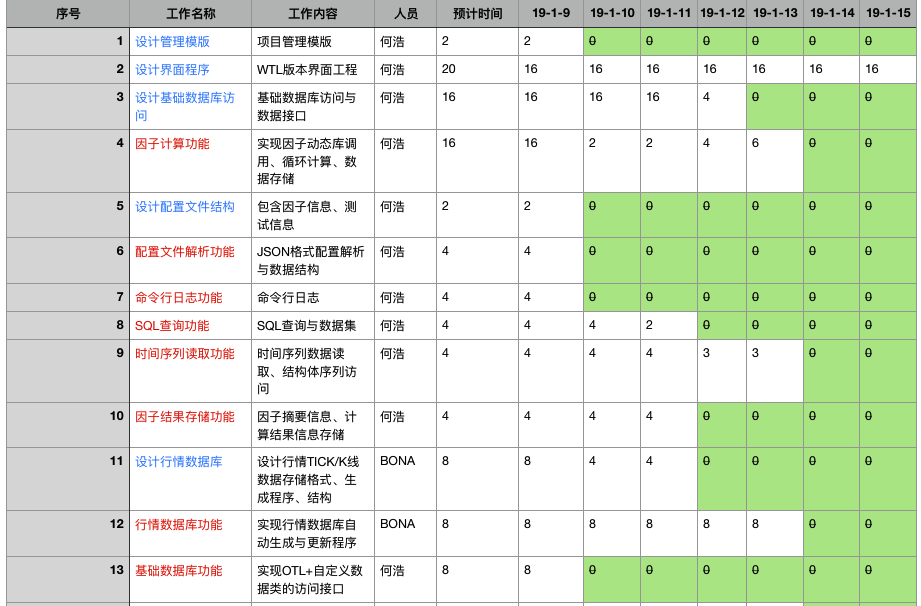
\includegraphics[width=5cm,height=4cm]{sprint1-backlog.png}
\label{fig:s1-p-backlog}
% \caption{LMAlpha系统sprint1工作任务表}
\end{minipage}%
}%
\subfigure[燃尽图]{
\begin{minipage}[t]{0.32\linewidth}
\centering
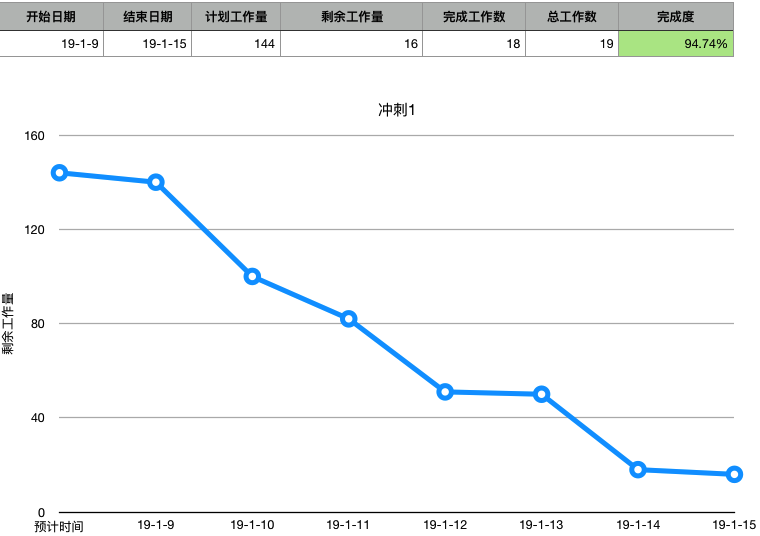
\includegraphics[width=5cm,height=4cm]{sprint1-burndown.png}
\label{fig:s1-p-burndown}
%\caption{LMAlpha系统sprint1燃尽图}
\end{minipage}%
}%
\caption{LMAlpha项目管理工具设计}
\end{figure}

%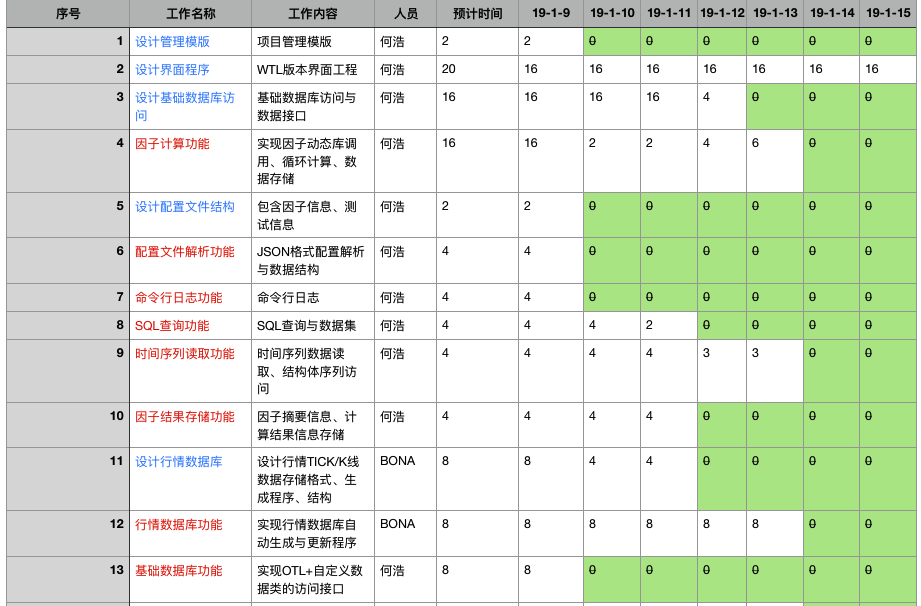
\includegraphics[width=7cm,height=6cm]{sprint1-backlog.png}
%\label{fig:s1-backlog}
%\caption{LMAlpha系统sprint1工作任务表}
%\end{figure}

%\begin{figure}[htbp]
%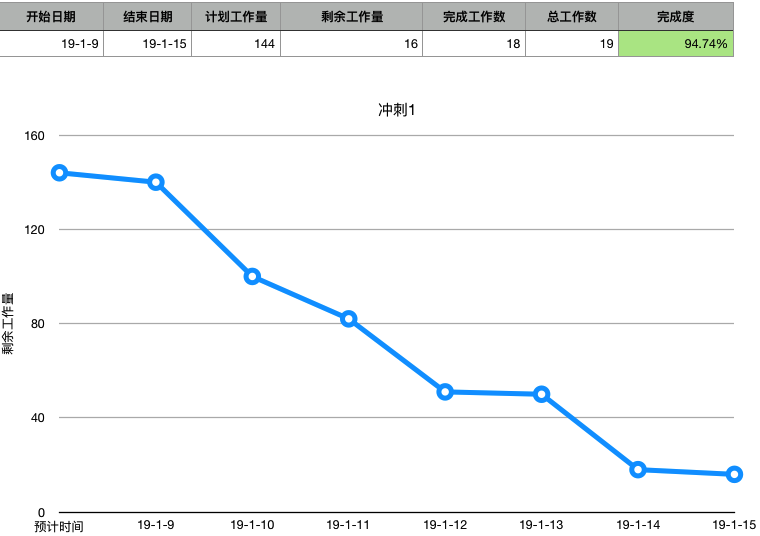
\includegraphics[width=7cm,height=6cm]{sprint1-burndown.png}
%\label{fig:s1-burndown}
%\caption{LMAlpha系统sprint1燃尽图}
%\end{figure}

    \chapter{数据库详细设计}
    \LARGE{BONA提供}\normalsize。
    \chapter{因子库详细设计}

\definecolor{codegreen}{rgb}{0,0.6,0}
\definecolor{codegray}{rgb}{0.5,0.5,0.5}
\definecolor{codepurple}{rgb}{0.4,0,0.92}
\definecolor{backcolour}{rgb}{0.95,0.95,0.97}

\lstset{language=C++,
backgroundcolor=\color{backcolour},
    commentstyle=\color{codegreen},
    keywordstyle=\color{magenta},
    numberstyle=\tiny\color{codegray},
    stringstyle=\color{codepurple},
    basicstyle=\footnotesize,
    breakatwhitespace=false,
    breaklines=true,
    captionpos=b,
    keepspaces=true}

\section{库初始化接口API}

从实践上,一个因子程序,只需要初始化一个因子库的实例。因子库初始化时,需要调用类lmapi构造函数。\\

\lstinline!auto api = new lmapi::lmapi();!\\

在使用完成后,需要调用其析构函数以完成资源回收。\\

\lstinline!delete api;!\\

使用C++智能指针可以简化初始化工作,并能够避免因为忘记释放而出现的内存泄漏问题。\\

\lstinline!auto api = std::shared_ptr<lmapi::lmapi>(new lmapi::lmapi());!\\

更进一步,使用高层API则完全避免因子库初始化的细节和具体工作,程序只需要在因子计算函数
开头设置初始化即可完成因子库的初始化工作。\\

\lstinline!LMAPI_INIT("cfg_name");//初始化因子库,打开配置文件!

        \section{控制台日志API}
        控制台日志类不能直接被初始化,因此如下调用会报编译错误。
\lstinline!auto log = new lmapi::console_log();!


        \section{配置文件读取API}
        \section{时间序列读取API}
        \section{SQL数据库查询API}
        \section{结构存储API}
    \chapter{辅助库详细设计}

    \LARGE{博文提供}\normalsize。
    \chapter{执行框架详细设计}
    \chapter{界面工具详细设计}
